
\documentclass[border=1pt]{standalone}
\usepackage[T1]{fontenc}
\usepackage{newtxtext}
\usepackage{newtxmath}
\usepackage{amsmath}
\usepackage{tikz}
\usepackage{pgfplots}
\usepgfplotslibrary{groupplots}
\usetikzlibrary{arrows.meta}
\pgfplotsset{compat=1.18}

\definecolor{cclassical}{HTML}{2166ac}
\definecolor{clearned}{HTML}{b2182b}
\definecolor{cproposed}{HTML}{1a9850}
\definecolor{cref}{HTML}{7f7f7f}
\definecolor{clight}{HTML}{67a9cf}
\definecolor{cbandlo}{HTML}{f4a582}
\definecolor{cbandhi}{HTML}{92c5de}

% Figure text is sized for a 252 pt column: axis labels a touch under the
% 8 pt caption size, tick labels one step below that.
\newcommand{\figlab}{\fontsize{7.5}{8.5}\selectfont}
\newcommand{\figtick}{\fontsize{6.5}{7.5}\selectfont}
\newcommand{\fignote}{\fontsize{6}{7}\selectfont}

\pgfplotsset{
  every axis/.append style={
    line width=0.5pt,
    scale only axis,
    tick style={line width=0.4pt, black},
    tick pos=left,
    grid=major,
    grid style={gray!30, line width=0.3pt},
    label style={font=\figlab},
    tick label style={font=\figtick},
    title style={font=\figlab, yshift=-2pt},
    legend cell align=left,
    legend style={
      font=\fignote, draw=black!35, fill=white, fill opacity=0.92,
      text opacity=1, inner sep=1.2pt, row sep=-1.5pt, legend image post style={scale=0.7}},
  },
  every axis plot/.append style={line width=0.7pt, mark size=1.3pt},
}
\begin{document}
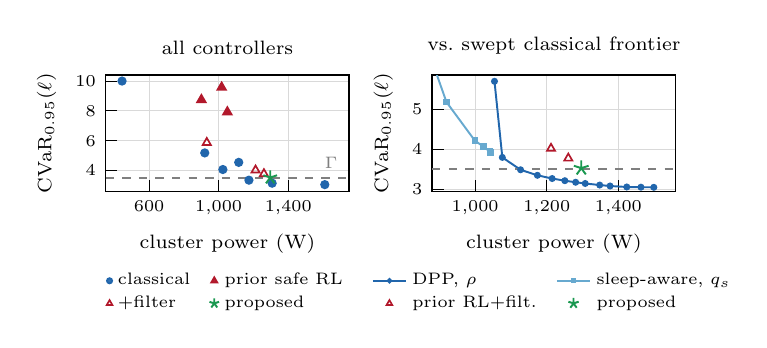
\begin{tikzpicture}
\begin{groupplot}[
  group style={group size=2 by 1, horizontal sep=30pt},
  width=88pt, height=42pt,
  xlabel={cluster power (W)},
  ylabel={$\mathrm{CVaR}_{0.95}(\ell)$},
  legend columns=2,
  legend style={at={(0.5,-0.62)}, anchor=north, draw=none, fill=none, font=\figtick, /tikz/every even column/.append style={column sep=5pt}},
]
\nextgroupplot[title={all controllers}, xmin=350, xmax=1750, ymin=2.6, ymax=10.4, xtick={600,1000,1400}, ytick={4,6,8,10}]
\addplot[only marks, mark=*, cclassical, mark size=1.3pt] coordinates {(1610,3.05008) (444.408,10) (1115.23,4.54372) (1173.79,3.34984) (1307.29,3.14567) (1024.03,4.06333) (919.903,5.17803)};
\addlegendentry{classical}
\addplot[only marks, mark=triangle*, clearned, mark size=1.7pt] coordinates {(1017.02,9.57374) (900.612,8.74058) (1049.84,7.91787)};
\addlegendentry{prior safe RL}
\addplot[only marks, mark=triangle, clearned, mark size=1.7pt, line width=0.6pt] coordinates {(931.56,5.8706) (1211.85,4.01922) (1260.1,3.77533)};
\addlegendentry{${+}$filter}
\addplot[only marks, mark=star, cproposed, mark size=2.6pt, line width=0.7pt] coordinates {(1296.33,3.52805)};
\addlegendentry{proposed}
\draw[cref, dashed, line width=0.6pt] (axis cs:350,3.5) -- (axis cs:1750,3.5);
\node[font=\fignote, text=cref, anchor=south east] at (axis cs:1740,3.5) {$\Gamma$};
\nextgroupplot[title={vs.\ swept classical frontier}, xmin=880, xmax=1560, ymin=2.95, ymax=5.85, xtick={1000,1200,1400}, ytick={3,4,5}]
\addplot[cclassical, mark=*, mark size=0.9pt] coordinates {(1054.01,5.69563) (1075.92,3.7963) (1126.79,3.4875) (1173.79,3.34984) (1214.96,3.26937) (1250.44,3.21514) (1280.67,3.17618) (1307.29,3.14567) (1347.76,3.1066) (1376.74,3.08276) (1423.48,3.05822) (1463,3.05312) (1498.92,3.05012)};
\addlegendentry{DPP, $\rho$}
\addplot[clight, mark=square*, mark size=0.9pt] coordinates {(732.035,10) (831.239,7.4244) (919.903,5.17803) (999.567,4.21063) (1024.03,4.06333) (1041.56,3.93392) (1043.43,3.9245)};
\addlegendentry{sleep-aware, $q_s$}
\addplot[only marks, mark=triangle, clearned, mark size=1.7pt, line width=0.6pt] coordinates {(931.56,5.8706) (1211.85,4.01922) (1260.1,3.77533)};
\addlegendentry{prior RL${+}$filt.}
\addplot[only marks, mark=star, cproposed, mark size=2.8pt, line width=0.7pt] coordinates {(1296.33,3.52805)};
\addlegendentry{proposed}
\draw[cref, dashed, line width=0.6pt] (axis cs:880,3.5) -- (axis cs:1560,3.5);
\end{groupplot}
\end{tikzpicture}
\end{document}
